% ---------------------------------------------------------------------------
% Based on the
% Author guideline and sample document for EG publication using LaTeX2e input
% D.Fellner, v1.15, Dec 14, 2018

\documentclass{egpubl}
 
% --- for  Annual CONFERENCE
% \ConferenceSubmission   % uncomment for Conference submission
% \ConferencePaper        % uncomment for (final) Conference Paper
% \STAR                   % uncomment for STAR contribution
% \Tutorial               % uncomment for Tutorial contribution
% \ShortPresentation      % uncomment for (final) Short Conference Presentation
% \Areas                  % uncomment for Areas contribution
% \MedicalPrize           % uncomment for Medical Prize contribution
% \Education              % uncomment for Education contribution
% \Poster                 % uncomment for Poster contribution
% \DC                     % uncomment for Doctoral Consortium
%
% --- for  CGF Journal
% \JournalSubmission    % uncomment for submission to Computer Graphics Forum
\JournalPaper         % uncomment for final version of Journal Paper
%
% --- for  CGF Journal: special issue
% \SpecialIssueSubmission    % uncomment for submission to , special issue
% \SpecialIssuePaper         % uncomment for final version of Computer Graphics Forum, special issue
%                          % EuroVis, SGP, Rendering, PG
% --- for  EG Workshop Proceedings
% \WsSubmission      % uncomment for submission to EG Workshop
% \WsPaper           % uncomment for final version of EG Workshop contribution
% \WsSubmissionJoint % for joint events, for example ICAT-EGVE
% \WsPaperJoint      % for joint events, for example ICAT-EGVE
% \Expressive        % for SBIM, CAe, NPAR
% \DigitalHeritagePaper
% \PaperL2P          % for events EG only asks for License to Publish

% --- for EuroVis 
% for full papers use \SpecialIssuePaper
% \STAREurovis   % for EuroVis additional material 
% \EuroVisPoster % for EuroVis additional material 
% \EuroVisShort  % for EuroVis additional material

% !! *please* don't change anything above
% !! unless you REALLY know what you are doing
% ------------------------------------------------------------------------
\usepackage[T1]{fontenc}
\usepackage{dfadobe}  

\usepackage{cite}  % comment out for biblatex with backend=biber
% ---------------------------
%\biberVersion
\BibtexOrBiblatex

%\usepackage[backend=biber,bibstyle=EG,citestyle=alphabetic,backref=true]{biblatex} 
%\addbibresource{egbibsample.bib}
%\usepackage{biblatex}
%\addbibresource{bib.bib}
% ---------------------------  
\electronicVersion
\PrintedOrElectronic
% for including postscript figures
% mind: package option 'draft' will replace PS figure by a filename within a frame
\ifpdf \usepackage[pdftex]{graphicx} \pdfcompresslevel=9
\else \usepackage[dvips]{graphicx} \fi


% WIS hack if you work in german
% \usepackage{ngerman}


\usepackage{egweblnk} 
% end of prologue

\title[EG \LaTeX\ Author Guidelines]%
      {Volumetric Ray Tracing}

% for anonymous conference submission please enter your SUBMISSION ID
% instead of the author's name (and leave the affiliation blank) !!
\author[Matthias Eberhardt]
%{\parbox{\textwidth}{\centering D.\,W. Fellner\thanks{Chairman Eurographics Publications Board}$^{1,2}$
 %      and S. Behnke$^{2}$
 {\parbox{\textwidth}{\centering Matthias Eberhardt$^{1}$
%        S. Spencer$^2$\thanks{Chairman Siggraph Publications Board}
        }
        \\
% For Computer Graphics Forum: Please use the abbreviation of your first name.
{\parbox{\textwidth}{\centering $^1$OTH Regensburg, Germany
%        $^2$ Another Department to illustrate the use in papers from authors
%             with different affiliations
       }
}
}
% ------------------------------------------------------------------------

% if the Editors-in-Chief have given you the data, you may uncomment
% the following five lines and insert it here
%
\volume{2021}   % the volume in which the issue will be published;
\issue{1}     % the issue number of the publication
% \pStartPage{1}      % set starting page


%-------------------------------------------------------------------------
\begin{document}


\maketitle
%-------------------------------------------------------------------------
\begin{abstract}

\end{abstract}  
%-------------------------------------------------------------------------

\section{Introduction}
In Computer Graphics, objects usually are represented as a set of geometric primitives ( e.g. triangles), displaying the surface of the object in question. However, this approach is not always suitable. For example, if the original data representation of the object is volumetric data (which might be produced by medical 3D-Scans [source!]), the traditional rendering technique would necessitate the creation of an intermediate surface representation that might introduce unwanted artifacts[Display of surfaces from volume data]. Another issue arises if the object has no well-defined surfaces, to which geometric primitives could be fitted, such as a cloud. In such cases, volumetric ray tracing might be used, a technique in which rays are cast through a volume which contains information about color and opacity, sampled at various points within the volume, accumulated and projected on a 2D-image (reformulate?). A description of this algorithm is presented in this paper, alongside several strategies for improving computational speed, such as (probabilistic) early termination of a ray, and sampling at lower resolutions within the volume.

\section{Basic Volumetric Ray Tracing Algorithm}
\subsection{Underlying Volume Data}
In this paper, we consider the topic of synthezisizing a 2d-image from a 3d-volume.
A volume can either be some continous, ternary function (such as perlin or simplex noise, which can be used to render volumetric clouds), or a discrete 3d array.
Similiar to a 2d-image which consists of pixels that can be adressed by a 2d vector $\vec{x} \in \mathbb{N}^2$, a 3d array consits of voxels that are adressed by a 3d vector $\vec{x} \in \mathbb{N}^3$. The color of a voxel at position $\vec{x}$ is called $c(\vec{x})$, the opacity $\alpha(\vec{x})$. The opacity is a scalar value, the color may also be a scalar value (for grayscale volumes), or a 3d vector (for colorful volumes). In the following, all values are assumed to be normalized to between 0 and 1. To project this volume to a image, for each pixel in the image, a ray is cast through the volume and sampled at multiple, evenly spaced points on the ray (see figure 1).
\subsection{Interpolation}
The sample points on the ray are in general part of $\mathbb{R}^3$. This is no problem if the volume is described by a continous function, which is defined everywhere. However if it is a discrete 3d array only defined for points in $\mathbb{N}^3$, the value of the volume at the sample point must be interpolated.
 This interpolation is done over the 8 closest voxels to the sample point (usually with a trilinear interpolation). The opacity values can be interpolated regularily, but the color values must be weighted with the respective opacity values before interpolation. To see why this is necessary, consider figure 2, which presents a simplified 2d example of a completly opaque, white object behind completly transparent empty space. Naively interpolating in this volume would result in two sample points, one completly white and opaque, the other gray and semitransparent. This gray point is not present in the original data and is an unwanted artifact. Weighting the colors with their opacity prevents this from happening.
 \subsection{Compositing Of Multiple Sample Points}
To compose the various sampled points on the ray to a single pixel, the points one after the other are alpha blended together. This compositing can be done front to back (starting with the sample point closest to the camera, blending it with the second, than the third, and so on), or back to front (vice versa).  Usually, the back to front approach is chosen, since it allows to optimize the computation (see below).
 TODO: formulas for blending, like in [Efficient Ray Tracing of Volume Data]
 In the following, $c(i)$ is the color of the i-th sample point, and $\alpha(i)$ the opacity. The accumulated opacity 
 \begin{equation}
 \beta(i) = 1 - \prod_{j=1}^{i}(1 - \alpha(j))
 \end{equation}
 is the fraction of light absorbed between the first and i-th sample point. The final color $c_f$, which is displayed in the projected image, is then
 \begin{equation}
 c_f = \sum_{i=1}^n((1-\beta(i)) * c(i))
 \end{equation}
 if the ray has n sample points.
\section{Optimization Strategies}
\subsection{Adaptive Termination Of Ray Tracing}
When looking at the compositing process described above, it becomes apperant that the contribution of a sample point to the final result decreases, the more other opaque sample points lie before it. For an extreme example, consider figure 3. Here, all sample points behind the fully opaque black wall contribute nothing to the final value and can therefore be ignored. In other words, going back to formula ???, the ray casting can be terminated after the accumulated opacity reaches 1, without changing the image quality. If some errors in the image are accceptable, the treshold value for terminating the ray tracing might be chosen to be somewhat lower, such as an opacity of 0.95.
\subsection{Ray Termination With Russian Roulette}
The above described by termination after a certain treshold is reached creates a bias in the synthesized image\cite{10.1145/97880.97886}. One way to avoid this is to use Russian Roulette to decide when to terminate a ray\cite{10.1145/147130.147155}. Unlike the above described approach,  Russian Roulette terminates a ray only with a certain likelihood once the accumulated opacity reached the treshold. The weight of the surviving rays is increased proportionally to compensate for the terminated rays.
\subsection{Pyramide Data Structures}
The following optimizations require a data structure called a pyramide. Similar to a set of mip-maps with decreasing resolutions, a pyramide is a set of volumes with decreasing resolutions. The different volumes of which the pyramide consists are called the levels of the pyramide. The lowest level (called level 0) is equal to the original volume. In general, level $n + 1$ is half the size of level $n$, and each voxel in level $n+1$ contains some information about 8 voxels in the lower volume. What information exactly is stored in the levels contains on what specific pyramide is used, of which there are multiple kinds. The first one is the so called average pyramide, which,a s the name suggets, stores the average of the 8 lower voxels in each voxel of the higher level (see figure).
\subsection{Presence Acceleration}
%-------------------------------------------------------------------------


\begin{figure}[htb]
  \centering
  % the following command controls the width of the embedded file
  % (relative to the width of the current column)
  %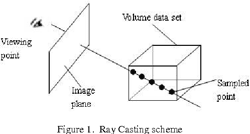
\includegraphics[width=.8\linewidth,natwidth=250,natheight=134]{RayCasting1.png}
  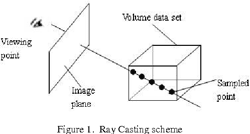
\includegraphics[width=.8\linewidth]{RayCasting1.png}
  \parbox[t]{.9\columnwidth}{\relax }~\cite{Appa2015RayCF}
  %
  \caption{\label{fig:firstExample}
          Illustration of the ray casting process.}
\end{figure}



\bibliographystyle{plain}
\bibliography{mybib}



%-------------------------------------------------------------------------
% bibtex
%\bibliographystyle{eg-alpha-doi} 
%\bibliography{bib}       

% biblatex with biber
%\printbibliography                

%-------------------------------------------------------------------------




\end{document}
